Behaviour of all entities within the game are discussed in this section.

\subsection{Structure}\label{subsec:behaviourStructure}
We have chosen to use goal-driven behaviour in our game.
Three main classes make up most of the structure, they are: \textit{Goal}, \textit{CompositeGoal} and \textit{AtomicGoal}.
As seen in the naming, a composite design pattern has been used to enable the grouping of goals while keeping the same functionalities.
This means that an \textit{AtomicGoal} can be used in the same way as a \textit{CompositeGoal} with the exception of \textit{AddSubGoal()},
which is only implemented in the composite.
This structure is used to create all strategy-level goals.

The class diagram below shows the structure (fig.\ref{fig:behaviourClassDiagram}).

\begin{figure}[h!]
    \begin{center}
        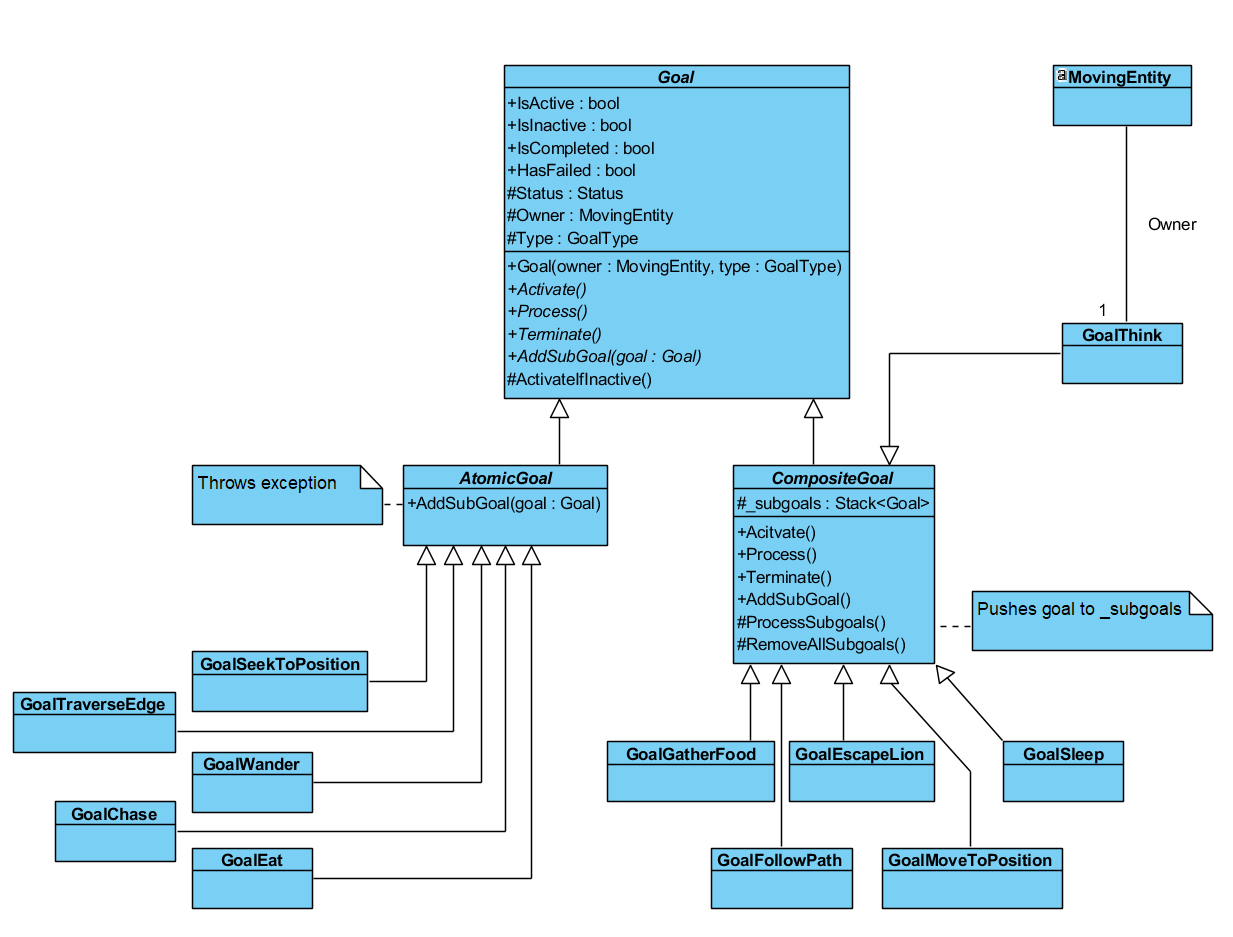
\includegraphics[width=40em]{Goals.png}
    \end{center}
    \caption{Goals class diagram}
    \label{fig:behaviourClassDiagram}
\end{figure}


\subsection{Goals}\label{subsec:behaviourGoals}
To give each entity a specific behaviour, we have created a couple of (composite) goals with some underlying atomic goals.
These goals wil be discussed below.

\subsubsection{Gather Food}\label{sec:behaviourFood}
Both the gazelles and the lions will have to gather food if they want to survive.
For gazelles it will mean that they have to find (\textit{GoalMoveToPosition}) grass or water and start eating.
Lions do not like grass, so they will have to chase (\textit{GoalChase}) a gazelle and eat it.
The gazelle will then try to escape (\textit{GoalEscapeLion}) which we will discuss in the next part.
If a lion caught a gazelle, the lion will eat (\textit{GoalEat}) the poor animal.

This is the most complex behaviour.
The \textit{GoalMoveToPosition} has as its first subgoal \textit{GoalSeekToPosition}.
This will continue until the path has been found and then \textit{GoalFollowPath} will be added with the found path.
While there is a path to follow, the \textit{GoalTraverseEdge} will be added, each time with a next node as position to travel to.
This enables the \textit{SeekBehaviour} to the given point.
If it is the last node, the \textit{GoalTraverseEdge} will start the \textit{ArriveBehaviour} to the final destination.

\subsubsection{Escape From Lion}\label{sec:behaviourEscape}
A gazelle does not want to be eaten by a lion, so it will try to escape a lion once it is within a certain range.
The \textit{FleeBehaviour} will be enabled for the gazelle, but its energy will drain.
%ToDo: Do we want flee or not, what should we do with this goal?

\subsubsection{Sleep}\label{sec:behaviourSleep}
Lions are actually lazy animals.
Once they had a nice meal, they want to sleep.
Gazelles will be very happy once that happens and they can relax for a while.
They will probably start grazing again as that is what they do most of the time.
If a lion sleeps, it won't do anything for a while, until he is fully back to strength.

This is a pretty simple goal, but very important for the lions.
It will temporarily disable all steering behaviour for the lion entity.

